% !TEX TS-program = xelatex
% !TEX encoding = UTF-8

\documentclass[a4paper,11pt]{article} % use larger type; default would be 10pt
\usepackage{../skills-analysis/default}
\usepackage{graphicx}
n
\ifxetex
\setmainfont{Droid Sans}
\setmonofont[Scale=0.9]{Droid Sans Mono}
\linespread{1.3}
\fi

\usepgfplotslibrary{fillbetween}

\title{Project Report --- Lumberjack}
\author{Joe MacMahon}
\date{\today}

\begin{document}
\maketitle

\section{Introduction}
\label{sec:introduction}
% TODO dot dot dot
As a part of my placement at CERN, I developed a software library called
Lumberjack over the course of several months.  This will be a critical
evaluation of that project, including [...], and also some surrounding context
of my placement itself.

\subsection{CERN Profile}
\label{sec:cern}
CERN, the European Organisation for Nuclear Research is a world-famous research
facility for particle physics located on the French-Swiss border, just outside
Geneva.  It was founded in 1954 (recently celebrating its 60th anniversary) and
currently has 21 member states from which it receives funding, and since that
time has been responsible for some of the world's most important achievements
in particle physics.

Such a large scientific operation obviously requires a substantial computing
infrastructure to support it, and as such CERN has made significant
contributions to the world of computing.  It is famous as the place where Tim
Berners-Lee created the first incarnation of the World Wide Web in 1991, and
more recently it has been known for developments in grid computing with the LHC
Computing Grid.

In terms of management structure, CERN is composed of a three-layer heirarchy:
there are eight departments\footnote{Beams; Engineering; Finance, Procurement
  and Knowledge Transfer; General Infrastructure Services; Human Resources;
  Information Technology; Physics and Technology}, each of which is divided
into a number of groups, and the groups are divided into sections.  My section,
for example, is IT-CIS-DLS, which means the IT department, Collaboration \&
Information Services (CIS) group, Digital Library Servces (DLS) section.
Ultimately the head of the organisation is the CERN council, which is made up
of delegates from each member state, and the day-to-day top-tier management is
undertaken by the Director-General, appointed for five years by the council.

% TODO talk about tech students

After a shutdown period of more than a year, CERN has just started the second
run of its principle particle accelerator, the Large Hadron Collider, colliding
particles at energies higher than ever previously observed.  This will mean
lots of publication and productive research activity over the coming months and
years and will continue to set the pace of global particle physics research.

\section{Context}
\label{sec:context}
My technical student project at centres on the CERN Document Server, which is a
service to manage papers, reports, press releases, bulletins and multimedia
created at CERN.  It also manages the library's loan system and journal
subscriptions, and provides access to peer-reviewed articles in high-energy
physics to CERN members.  The software that runs CDS is called Invenio, and
also powers a family of other sites as well, for example Inspire and Zenodo.

As with many other large services, a system for gathering and visualising usage
data is important.  In Invenio version 1 this is achieved by logging event data
to MySQL and then generating graphs serverside viewable by an administrator,
however this approach doesn't scale well when a service grows to the size of
CDS.  So, my project is to implement a new system for usage data and analytics
based on Elasticsearch, which is a distributed data store and search engine.

The scope of this report concerns the logging aspect, although my overarching
project also includes implementing visualisations of the logged data.

Since Invenio is written in Python, we decided on using the standard Python
logging system to collect our event data.  It's easy to use since it avoids
lots of object-passing; it's a standard and therefore stable and well-tested;
plus its heirarchical logging system enables us to keep logs going to
Elasticsearch within their own namespace, to make sure ordinary debug or
warning logs stayed out of the Elasticsearch ecosystem.

\subsection{Outline of Python Logging}
\label{sec:pythonlogging}
A brief outline of the Python logging system.

\begin{figure}[H]\centering
  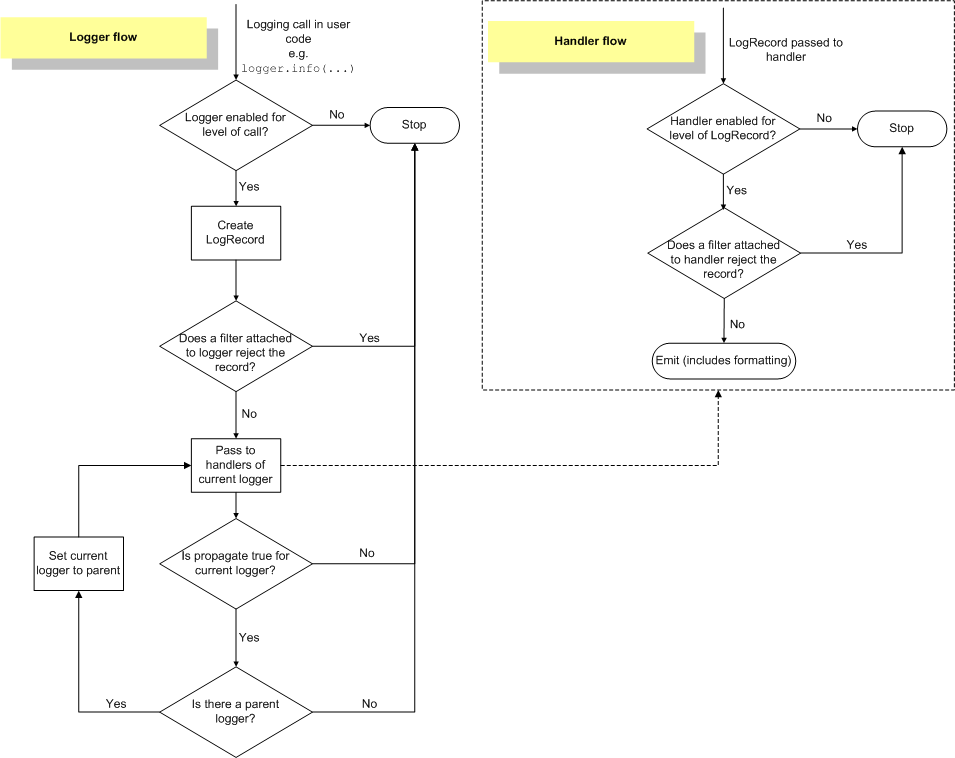
\includegraphics[width=\textwidth]{logging_flow}
  \caption{The flow of log event information.\protect\footnotemark}
\label{fig:pythonlogging.flowdiagram}
\end{figure}
\footnotetext{Copyright Python Software Foundation; PSFL licence.  Source: \url{https://docs.python.org/2/howto/logging.html}}

However, the Python logging system has no in-built compatibility with
Elasticsearch, and at the time there were no third-party libraries to connect
the two systems.

\subsection{How Elasticsearch stores data}
\label{sec:elasticsearch}
A brief outline of Elasticsearch indices inc. time-based-ness, maybe mappings

\section{Proposal}
\label{sec:proposal}
Faced with this issue, we decided it would be a good idea to develop our own
library to do connect the two systems.  It would provide a handler to attach to
a logger in the heirarchy, and forward events expressed as Python \texttt{dict}
objects to Elasticsearch over the REST API.  It should also be tolerant to use
cases other than our own by accepting standard string-based log messages.

% TODO maybe take this line out?
As it later turned out, the  it would also need to maintain an internal queue of
events, and flush the entries to Elasticsearch asynchronously

\section{Implementation}
\label{sec:implementation}
In this section, we will give an overview of how the library works, and then
move on to an in-depth look at a selection of aspects.

\subsection{Outline of Lumberjack}
\label{sec:implementation.lumberjack}
The crux of the library is to provide a \texttt{LogHandler} object which will
send events that it receives on to Elasticsearch.  This is attached to a
\texttt{Logger} object on application setup, and then events are passed to this
\texttt{Logger} in the standard way.  Lumberjack needs to know what
Elasticsearch index to send data to, so we use a factory pattern to generate
parametrised \texttt{LogHandler} objects.  We then attach these to the
\texttt{Logger} at the root of our particular namespace.

In Python pseudo-code:
\begin{lstlisting}[language=Python,basicstyle=\ttfamily]
import logging
import lumberjack
lj = lumberjack.Lumberjack( ... some global initialisation parameters ... )

myHandler = lj.getHandler(index='my-elasticsearch-index')
myLogger = logging.getLogger('some_namespace')
myLogger.addHandler(myHandler)
\end{lstlisting}

\begin{figure}[H]
  \centering
  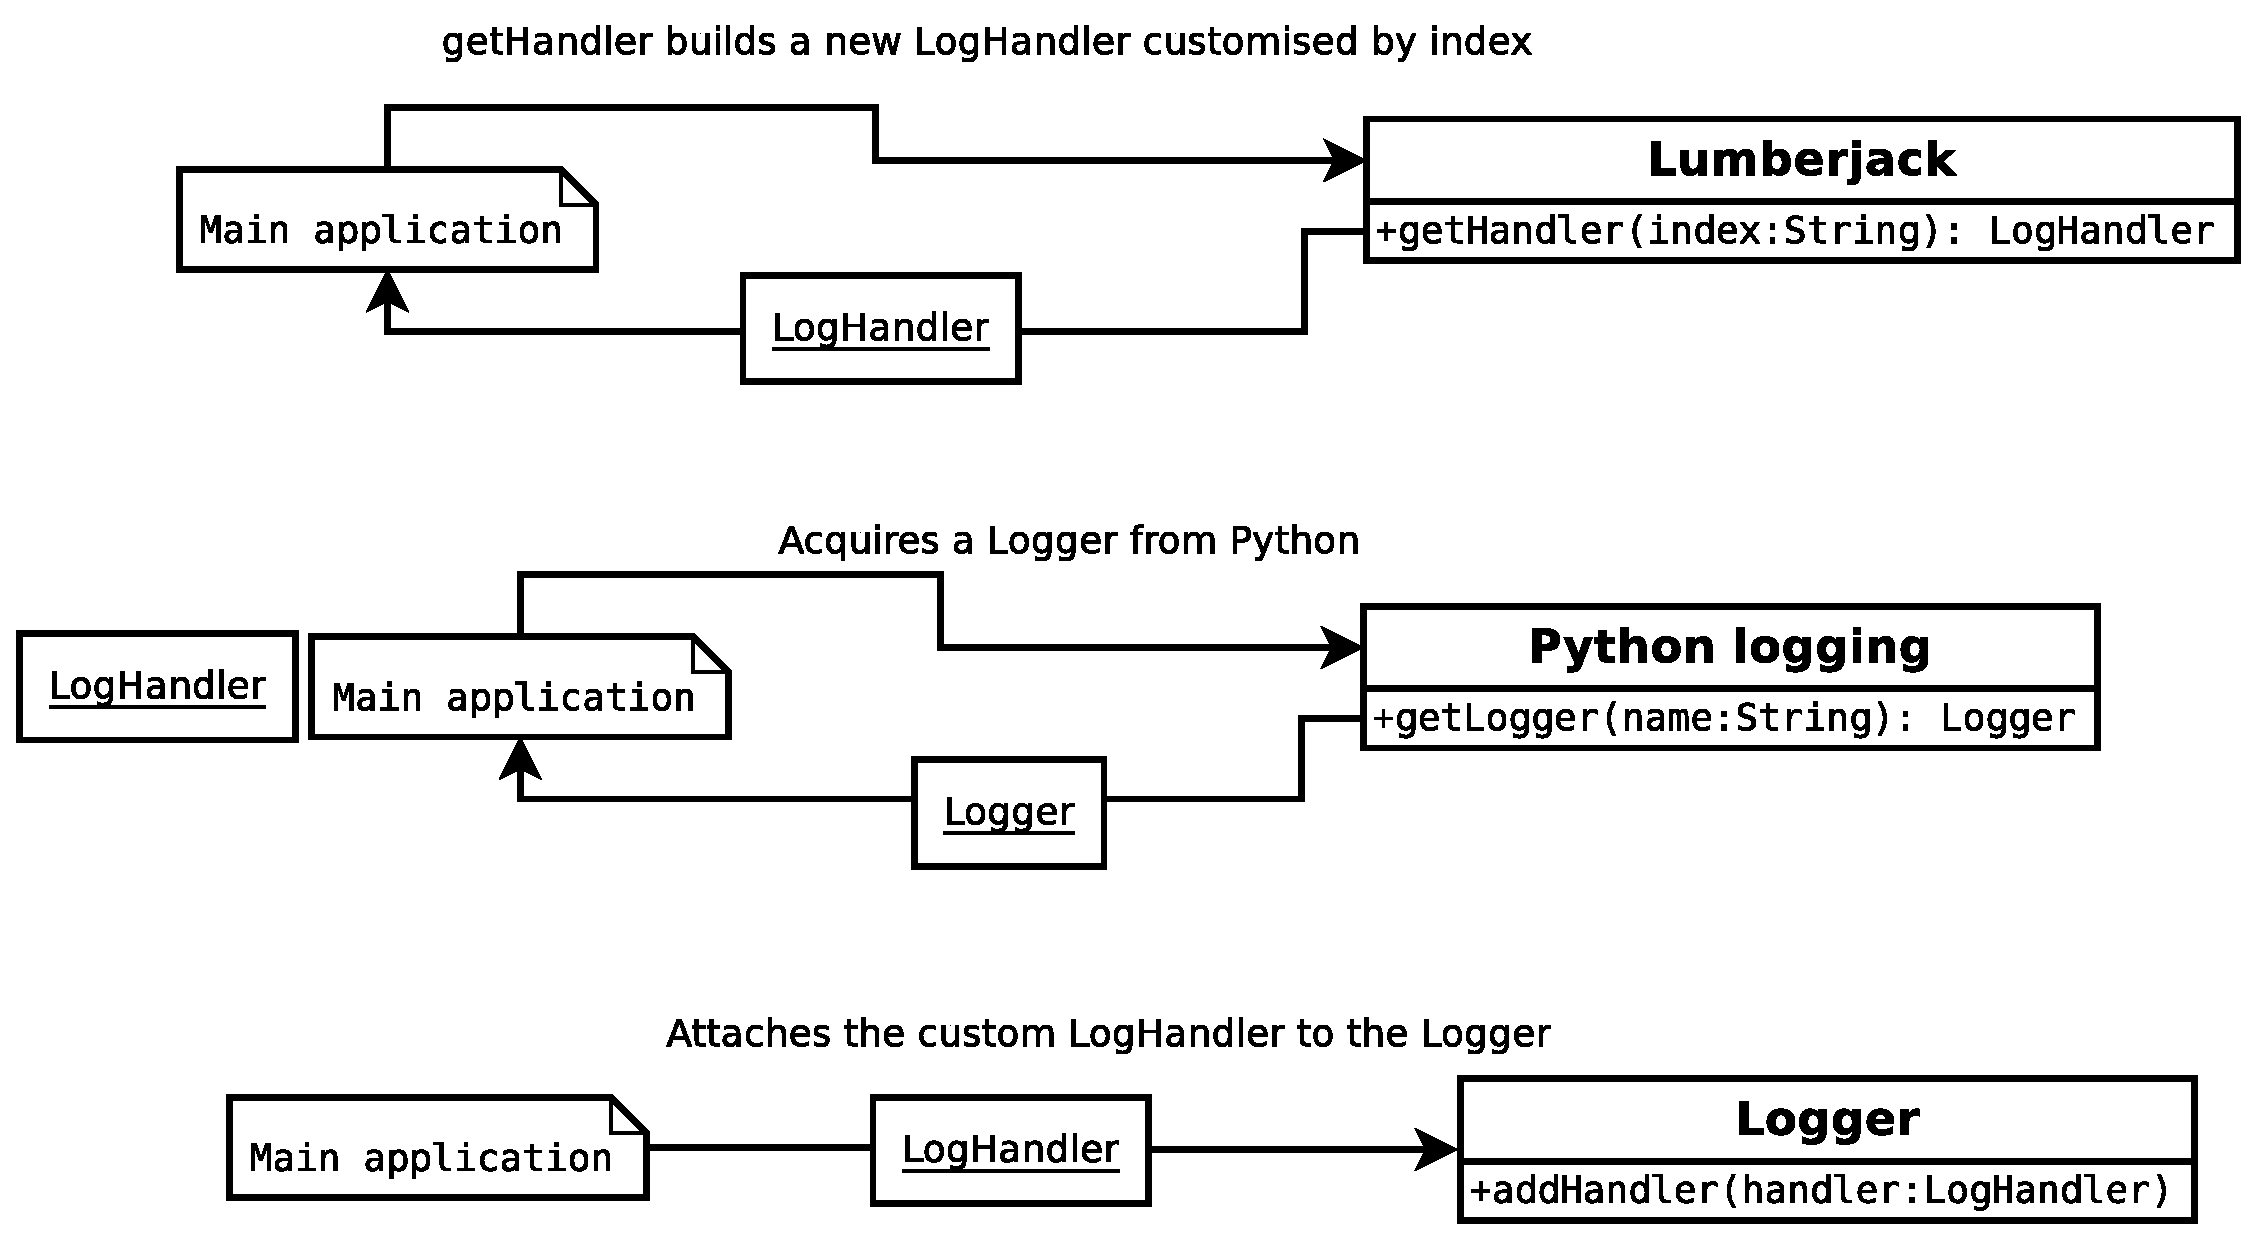
\includegraphics[width=\textwidth]{initialisation_step}
  \caption{Initial process for attaching a Lumberjack handler to a Python Logger}
  \label{fig:implementation.initialisation_step}
\end{figure}

Once initialisation is finished, the main application should then use the
standard \texttt{Logger} methods, \texttt{.info()}, \texttt{.warn()}, etc., to
pass an event into Elasticsearch.  The custom log handler adds some metadata
(timestamp, severity level, logger name), and sends the augmented event data to
Elasticsearch.  To do this it uses the official Python Elasticsearch interface
library.

Again in Python pseudo-code:

\begin{lstlisting}[language=Python,basicstyle=\ttfamily]
import logging

event_A_logger = logging.getLogger('some_namespace.event_A')
event_B_logger = logging.getLogger('some_namespace.event_B')

event_A_logger.info({'data': 1})
# Will index {'data': 1, '@timestamp': 1434120117, 'level': 10,
#             '_type': 'some_namespace.event_A'}
\end{lstlisting}

\subsection{Indexing}
\label{sec:implementation.indexing}
The straightforward approach to getting the data for an event from the
\texttt{LogHandler} to Elasticsearch would be to simply place, the handler's
\texttt{.emit()} method, a call to the \texttt{.index()} method of the global
Elasticsearch singleton.  This would result in the following simplified call
stack:
\begin{enumerate*}
  \item logging.Logger.info()
  \item lumberjack.Handler.emit()
  \item elasticsearch.Elasticsearch.index()
  \item elasticsearch.Transport.perform\_request()
  \item urllib3.HTTPConnectionPool.urlopen()
\end{enumerate*}

A problem arises in the fact that the last method on the call stack,
\texttt{.urlopen()}, will block until a response from the cluster is received.
After some benchmarking and profiling, we established that under our
circumstances this blocking could take 300-400 ms, which was unacceptable to
our situation of performing 3-4 logging operations per single page load.  In
fact, logging operations should generally disrupt the main application as
little as possible, so clearly this presented a problem.

In the Elasticsearch Python library, there is a method \texttt{.bulk()} which
allows bulk-indexing of events to Elasticsearch.  Since this eliminates a lot
of the overhead, using the bulk indexing results in a much lower per-event
latency from Elasticsearch.  Thus, one initial solution proposed was to
maintain a queue of events to be indexed, and on every (say) 500th event added,
we would flush the queue into Elasticsearch.  This bulk operation would still
carry a latency of around 400 ms, but it would only occur once every 500 log
events.

While this solution provided on average a much more efficient solution, it had
a number of problems: the `every 500' rule would have caused seemingly random
latency spikes in logging operations, and in slow periods the flushing of the
queue would have been much less frequent than in periods of high-activity.

So, in the end we decided to implement a completely asynchronous queueing and
flushing mechanism using the Python threading library.  A new singleton class,
\texttt{ActionQueue}, was added, which runs in a separate thread.  Events are
passed to it and added to an internal queue, which is then emptied and flushed
to Elasticsearch in bulk every 30 seconds or 500 events, whichever is sooner.
Both of these settings are configurable, and threading locks are used to make
emptying and adding to the queue atomic operations, thereby eliminating race
conditions that could cause events to be lost.

% TODO maybe expand on threading

%- async/queue, benchmarking
%- http libraries
%- threading

\subsection{Testing}
\label{sec:implementation.tdd}


- tdd
- mock

- schemas?
- fallback
- nginx?
- documentation

\subsection{Future Considerations}
\label{sec:future}
- rabbitmq
- py.test

\section{Useful Links}
\label{sec:references}

\begin{description*}
  \item[CERN] \url{http://cern.ch}
  \item[CERN Document Server] \url{http://cds.cern.ch/}
  \item[Elasticsearch] \url{https://www.elastic.co/products/elasticsearch}
  \item[Elasticsearch Python] \url{https://github.com/elastic/elasticsearch-py}
  \item[Inspire] \url{http://inspirehep.net}
  \item[Kibana] \url{https://www.elastic.co/products/kibana}
  \item[Lumberjack] \url{https://github.com/jmacmahon/lumberjack}
  \item[Python Logging System] PEP 282, \url{https://www.python.org/dev/peps/pep-0282/}
  \item[Python Threading Library] \url{https://docs.python.org/2/library/threading.html}
  \item[Zenodo] \url{http://zenodo.org}
\end{description*}

\end{document}